\section{Implementation of \pdht}


The \pdht system implements a distributed, PGLAS key/value store that
is asynchronously accessible through one-sided {\em insert}, {\em
  read}, {\em write}, and {\em atomic update} operations.  \pdht uses
a hash function to map an arbitrary user-supplied key (i.e. a logical
address) to a process rank and 64-bit hash value, giving each key a
deterministic physical location within the distributed hash table.

A \pdht structure is treated as a distributed array of objects, with
partitions spanning all processes. Upon the creation of a new
distributed hash table, \pdht allocates two portal table
entries (PTEs). The first PTE contains the {\em pending} match list and the
second contains the {\em active} match list. The pending match list is
populated with a number of entries that match any incoming
communication requests (i.e. a wildcard). Each ME in the pending list
corresponds to a single entry in the local portion of the distributed
array. MEs in the pending list are marked as use-once and are unlinked
after being written to, whereas MEs in the active list can be marked as either
use-once or persistent, depending on the usage model.

The principal idea in \pdht is to create a match list entry (ME) for
every element in the hash table. The 64-bit hash value produced by the
hash function is used as the value for the match bits field that is provided
to Portals put and get operations. By using the hash value as
the match bits field, the handling of a get operation can be
handled entirely by the Portals implementation.

% TODO --
%\pdht's usage of the Portals matching interface differs from MPI in several important ways: ...

\subsection{Insert Operation}

When adding a new key/value object to the hash table, the key is
hashed, giving both the target processor rank as well as the match
bits field to be used for the entry. In the case of a local insertion,
the initiating process can copy the entry into the hash table array and
locally insert a new ME with the match bits set to the hashed value. 

When the entry hashes to a remote process, the initiating process
performs a one-sided put operation onto the pending PTE, consuming one
of the wildcard ME entries on the match list. The hash entry data is
transferred and stored into the array entry that is associated with
the pending entry. As shown in Figure \ref{fig:put} (b), at this point
the table entry data resides in the correct location on the target
process, but the match lists are in a transition state.  To complete the
operation, a new wildcard ME must replace the consumed entry on the
pending list. Additionally, the active list must be updated with an ME
that contains the hash. Completion of these actions results in the state shown
in Figure \ref{fig:put} (c).

\begin{figure*}
  \centering
  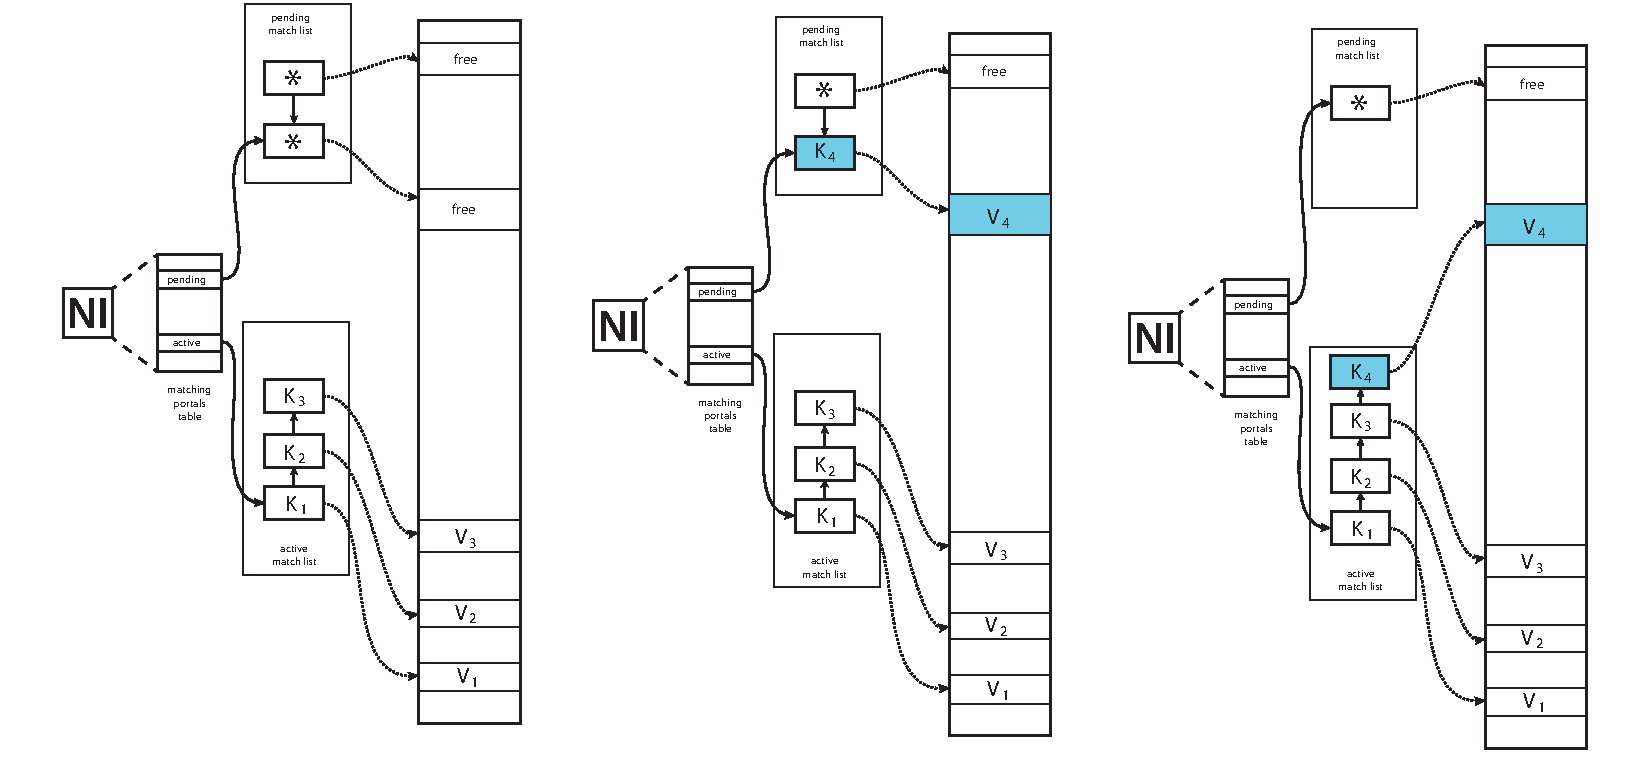
\includegraphics[width=\linewidth]{figs/put}
  \caption{Sequence of target-side actions performed during a \pdht~{\tt insert()} operation.}
  \label{fig:put}
\end{figure*}

The current approach to handle the match list management between the
pending and active lists is to use a dedicated progress thread. This
thread blocks on the event queue associated with the pending PTE,
and is automatically notified by the Portals layer when an insert request
arrives. As insert requests are received, the
progress thread replaces the consumed wildcard ME on the pending list and allocates a
new pending list entry buffer. The thread also creates a new
ME with the appropriate match bits set and appends it to the active
list. Subsequent data access operations will find a match in the active list.

\subsection{Data Access Operations}

One-sided read, write, and atomic update operations are handled by
computing the hash function on the key, then performing corresponding
one-sided Portals get, put, or atomic operation, using the process
rank and match bits provided by the hash. If the operation is unable
to find a matching entry on the active match list, the operation
reports a not-found message. If the key of the retrieved table entry
doesn't match the requested key, \pdht notes the collision and either
returns control to the application or performs a linear probe,
depending on the desired behavior.

\subsection{Collisions and Key Sparsity}

Collisions occur when multiple keys map to the same rank/hash pair.
In the case of a collision,
PDHT utilizes a linear probing solution. The library can
also be configured to simply detect collisions and let the application
take an appropriate action.
% JSD: How does linear probing work?
% DBL:
% pdht_get(key,...): -> 
% while (!found) {
%    PtlGet(match, pte, rank, data, ...)
%    if (data.key != key) { match = match+1; }
% }

A significant difference between traditional hash tables and \pdht is
that using the Portals match list for table entries detaches the link
between the computed hash code and the actual location in
memory. Typically, a hashed key, $K$,  is used with modular arithmetic to
determine a location in an array of size $N$. The hash function
provides a mapping between $|K| \rightarrow N$ elements. When $|K|$ is
much larger than $N$, the likelihood of collisions increases. In order
to manage collisions, hash tables typically store a list of objects within
each array entry.
% JSD: The set of processes sort of takes the place of the array?
% 
% DBL: the set of processes + set of match bits takes place of the array
%
% traditional: hash(key) -> bucket in |0..N-1| -> array[bucket]
%
% pdht: hash(key) -> rank,bits in |NP * 2^64| -> ME
%           each ME -> array[bucket] at creation time via insert or
%           polling thread

\pdht also uses an array to hold the collection of hash table
entries, but the indexing into this array is performed indirectly,
through the ME in the match list. A \pdht hash function provides the 
mapping: $|K| \rightarrow P \times 2^{64}$. Each key is mapped to one
of $P$ distinct process ranks and a unique 64-bit match bits
value. Compared to traditional implementations, $N \ll  P \times
2^{64}$, which has the impact of dramatically reducing the likelihood
of a collision, provided a reasonable hash function.


%%% Local Variables:
%%% mode: latex
%%% TeX-master: "paper"
%%% End:
